\section{Question Formulation}
Given a graphical model designed to perform statistical analysis upon a PDB and the uncertainty associated with a set of unobserved nodes, the main task of CrowdPillar is designating which nodes to observe and by performing inference reduce the uncertainty of the entire system.  Observation is the act of clamping a random variable to a specific value.  For the case of information extraction, this is label provided by the crowd.

This section is concerned with precisely how to select the optimal node to observe from a graphical model.  The node whose resolution best reduces the overall model uncertainty is the one sent to the crowd.  Before we can form a discussion about optimal node selection, we must first introduce the metric by which uncertainty is measured in our sysem.

\subsection{Total Utility Function}
In order to make a decision about which node to query, we develop the concept of a Total Utility Function (TUF). The TUF fulfills two prominent and necessary roles: quantification and selection.  At its core, it represents a quantification of the uncertainty so that we may measure differences in total uncertainty between different configurations of our model.  The second functionality is that is designed in such a way as to rapidly promote uncertainty reduction by identifying the key node hubs whose resolution gives the greatest effect.  Node features such as entropy and dependency need to be taken into account and will be discussed in greater detail later in the section. 

There are two paradigms that may be used here.  The first is to assign each node $t$ a score $S_{t}$ in a simple manner and combine them in some complex model-dependent way.  The other is to leave the score combination simple. but create complex ways to attach a score to each node.  We choose the latter approach because it is more easily generalizable to various PGMs.

The simplest way to combine scores is to take the sum, ie. for a model with T nodes:
\begin{equation}
TUF = \sum_{t=1}^{T}S_{t}
\end{equation}
This makes node selection for uncertainty reduction simple.  By observing the node with the highest score and reducing that score to zero, the entire function is maximally reduced.  The tradeoff is that the method of assigning a score may be much more complex.  We devote the remainder of this section to discussion of the various techniques for assigning a score and settle on a combined metric that we assert can be used for a wide range of probabilistic graphical models.

\subsection{Simple Methods of Assigning Scores}
Below we present two methods of attaching scores to nodes based on their marginal entropy and dependency among other nodes.  The main application of these methods is to linear-chain conditional random fields, but additional model dependent methods may be used in the appropriate context.  

\subsubsection{Marginal Entropy}
Linear-chain Hidden Markov Models or Conditional Random Fields are one the simplest type of PGM to assign a score to due to the uniformity of each node in the graph.  With the exception of the first and last nodes in the chain, every node has the same type and number of pair-wise edge features.  Thus any means of assigning $S_{t}$ is consistent across all nodes.

The property we hope to achieve with score assignment is to give the largest scores to the most uncertain nodes.  The uncertainty associated with a specific node is achieved by calculating the entropy over its marginalized distribution.  Marginalization in a CRF is done through the forward-backward algorithm \cite{Lafferty01} utilizing forward ($\alpha$) and backward ($\beta$) inference messages meeting at the marginalized node.  The marginal probability of a node $t$ in the sequence being assigned label $i$ is given by
\begin{equation}
p(\mathbf{Y}_{t}=y_{i}|\mathbf{x}) = \frac{\alpha_{t}(y_{i}|\mathbf{x})\beta_{t}(y_{i}|\mathbf{x})}{Z(\mathbf{x})}.
\end{equation}
The marginal entropy of node $t$ is then
\begin{equation}
H_{t} = \sum_{i=1}^{L}p(\mathbf{Y}_{t} = y_{i}|\mathbf{x})log[p(\mathbf{Y}_{t} = y_{i}|\mathbf{x})],
\end{equation}
where L is the label space of the problem.  This leads to a simple uncertainty score assignment of $S_{t}=H_{t}$.

In making a decision about which node in a sequence of length $T$ to the submit to the crowd, we calculate the marginal entropy $H_{t}$ for every node and take the highest one,
\begin{equation}
Selection = \argmax_{t}(H_{t}) \hspace{0.5in} t=1,\dots,T.
\end{equation}
The crucial assumption here is that the most uncertain node generally has the highest probability of being incorrect compared with other nodes in the sequence.  In our experiments in Section 6 we show that this is a safe assumption to make.  

Although the response from the crowd only holds information pertaining to a single node's assignment, inference provides a wider-reaching chain reaction effect.  As discussed earlier, the most likely path sequence is determined by a type of Viterbi dynamic programming algorithm.  After clamping the label of node $t$ to label $i$, we run a Constrained Viterbi \cite{Kristjansson:2004:IIE:1597148.1597216} which fixes the Viterbi path to run through $i$ at $t$.  This may change the labels of other nodes in $t$'s neighborhood compared to before clamping.  Thus the total entropy of the entire sequence may be reduced well beyond the contribution of the selected node.

\subsubsection{Most Dependency}
Since inference provides a means of updating multiple nodes from a single answer, it would be useful to have a score that is proportional to this chain reaction effect.  That is, those nodes with the greatest ability to impact its surrounding neighborhood should be awarded the highest score.  This increases the impact of every question asked. 

For generalized graphical models, it is clear the impact of resolving a node is proportional to the number of nodes which share edge-wise features with it.  Nodes with a higher degree are more "important" to resolve.  Thus another metric for scoring can be the degree of each node,
\begin{equation}
SELECTION = \argmax_{t}(deg(V_{t})) \hspace{.2in} t=1,\dots,T.
\end{equation}

To illustrate this idea further, consider an experiment involving a connected social network and movie recommendation system.  We want to select a single user to ask about which movies they like and in turn make recommendations to their friends under the assumption that friends like similar movies.  The user likely to give the maximum number of recommendations is simply the one with the most friends.  Modeling the social network as a graph, this is the node with the most connections.

This score assignment based on the node with the highest dependency can also be used in the information extraction domain.  One recent modification to the linear-chain model is to use "skip-edges" \cite{Sutton04} connecting possibly distant nodes in the sequence.  The goal is for multiple nodes representing the same entity to be resolved simultaneously.  In this case we would seek to ask a question about the nodes connected by the greatest number of skip-edges, ie. resolving those entities that appear most in the sequence and whose resolution has the greatest impact.

\subsection{Neighborhoods: Total Score Metric}
It is desirable to be able to assign a score to a a node in a generalized probabilistic graphical model without explicitly depending on the type of model, eg. linear-chain vs. skip-chain.  The two factors by which a score can be measured are the entropy of the node and its degree.  To this end, we propose a method that combines both properties and can be applied to a numerous models more general than the linear-chain discussed in detail in this earlier in this section.

\begin{figure}
\centering
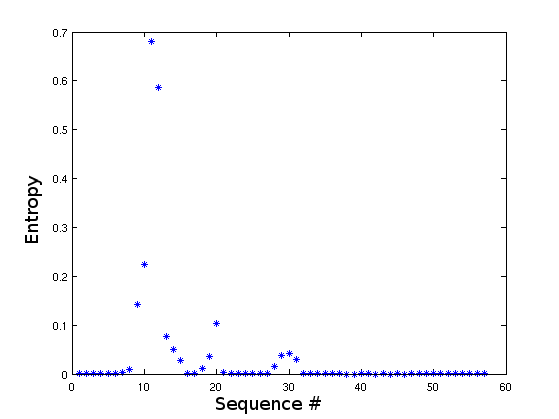
\includegraphics[width=0.9\linewidth]{images/ent_dist1.png}
\label{fig:ent}
\caption[example]{The entropy distribution for a sample bibliographic sequence.}
\end{figure}

Figure \ref{fig:ent} shows the entropy distribution for the labeling of a sample bibliographic sequence.  Rather than being randomly distributed, high entropy values appear in pockets of small neigborhoods.  This is standard among many sequences investigated.  This notion of clustering of high entropy nodes around the highest ones in the sequence motivates an additional method of combining scores that naturally carries the properties needed from the previous two sections.

Instead of taking the marginal entropy over a single node as the only score metric, we combine the entropies of each node with those of all nodes of order $K$ or less.  By this we mean all nodes connected to the node in question by $K$ or fewer edges.  Formally:
\begin{multline}
S_{t} = \sum_{i=1}^{L}p(\mathbf{Y}_{t} = y_{i})log[p(\mathbf{Y}_{t} = y_{i})]\\
+\sum_{k=1}^{K}\sum_{j=1}^{L}p(\mathbf{Y}_{t+k} = y_{j})log[p(\mathbf{Y}_{t+k} = y_{j})]\\
+\sum_{k=1}^{K}\sum_{m=1}^{L}p(\mathbf{Y}_{t-k} = y_{m})log[p(\mathbf{Y}_{t-k} = y_{m})]
\end{multline}
In our experiments we take $K=1$ and analyze all nodes connected by a single edge.  Again $SELECTION$ is the node with the max $S_{t}$.

As per Figure \ref{fig:ent}, this should have little effect on the single highest marginal method for linear-chain models.  The highest entropy node in a sequence usually appears among other high entropy nodes.  In addition, for models with greater variation in connectivity, nodes with a larger neighborhood will generally have a larger score by the Neighborhood Metric.  This method automatically accounts for the tradeoff between node pockets of high entropy and others that are connected to a larger number neighboring nodes.  Currently, we only cover linear-chains CRFs, but we plan to apply this method and conduct experiments on other models such as Bayesian Networks in our future work.
